\documentclass[12pt,b5book]{extarticle}

\usepackage{xltxtra}
\setmainfont[Ligatures=TeX]{IPAPMincho}
\setsansfont{IPAPGothic}
\setmonofont{IPAGothic}
\XeTeXlinebreaklocale "ja"
\usepackage{hyperref}
\usepackage{graphicx}

\begin{document}
\section{Pietの自動生成}

\subsection{はじめに}

こんにちは、NoNameA 774です。
KMC(京大マイコンクラブ)というPietサークルに入っているのですが、
サークルの人々がPietを手で(書いてる\textbar{}描いてる)のを見て、
絵としての意味を持つ方法以外でPietを人間が描くのは不毛だと思い、
Pietの自動生成を行いたいと思った次第です。
今回一度ぐらいサークル参加をしてみたいとコミケに初申し込みしてみたら、
運良く当選したのでこの本を書いている次第です。

前回のコミケ(C88)でも同じようなペーパを出したので(\url{https://nna774.net/piet/})、
それの続きのような感じです。
前回のペーパは二日目のアース・スター作品のゾーンに割り当てられた友人のサークルにて配布したのですが、
完全にアウェーな中でも何枚か配ることに成功しました。
もしその際手にとってくださった方がいれば、ありがとうございました。

KMCの部誌の記事としてこの本を出さなかった意味はあるのか、という話もありますが
(今回KMCの部誌の記事として遠野へ旅行した旅行記を書きました。
今これを読んでる時点ではほぼ手遅れである可能せが高いですがそちらもよろしくお願いします)、
一度自分のサークルで参加したかったということでよろしくお願いします。

\subsection{前提}

今回この記事はプログラミング言語Pietについて書いているので、
Pietそのものについての解説もすべきな気がするのですが、
ここでは概要を説明するに留めます。

Pietについてより詳しくは公式サイト(\url{http://www.dangermouse.net/esoteric/piet.html})を見るなり、
うちの部員の書いたスライド(\url{http://www.slideshare.net/KMC\_JP/piet-46068527})を参照するなどお願いします。

また、このスライドに書かれているPietのエディタですが、
現在OSSになっていて\url{https://github.com/kndama/Pidet}から入手可能となっています。
Pietを触ってみよう という方はこれを使うか、
とりあえず試してみるだけならPietDev(\url{http://www.rapapaing.com/blog/?page\_id=6})を利用するのが良いと思います。

あとこれはPietに関係ないのですが、
上記のスライドに出てくるUnambiSweeperですが、
現在作者によりアンドロイドアプリとしてリリースもされているので(\url{https://play.google.com/store/apps/details?id=jp.nobody.dnek.unambisweeper})、
ぜひダウンロードして見てあげてください(宣伝)。

\subsubsection{言語仕様の概要}

Pietは20色の色で絵を描くことによりソースを書きます。
赤、黄、緑、シアン、青、マゼンタの6色と、
それに明、普通、暗の三種類を組み合わせた合計18色に白と黒を合わせた合計20色です。
この色と明度はこの順序で後述する差を考えるときには扱われます。

この20色で書かれた図形の上を最初は左上にあるプログラムポインタが、
DirectionPointer(以下DP)、CodelChooser(以下CC)と呼ばれる2つのステートを参照しながら移動していくことにより命令を実行します。
このプログラムポインタの動き方を説明するのはすこしややこしいので詳細はスライドを参照して欲しいのですが(23-29枚目のところです)、
簡単に言うとDPが上下左右の方向を指し、
CCがDPの指す方向を向いた時の右左を指定します。
プログラムポインタはDPの方向を向き、
今いるマスと同色のマスの中で一番その方向に遠いマスを探します。
複数ある場合がその中でCCで指定された方向に一番端のものを探し、
その一つ前のマスに移動します。

この移動の時に、移動元と移動先の色の``差''と、
移動元の面積により命令が決定されます。
6色の差と3明度の差(それぞれ循環して考えます。赤から緑の差は2段階で、緑から赤の差は4段階。明から暗は2段階、暗から明は1段階)により、
17個の命令が定まっています。

それぞれの命令の割当は省きますが、
Pietはこれらの命令によりスタックを操作するスタック指向プログラミング言語となっております。
おおまかに分類するとスタック操作、四則演算、否定、比較、CCとDPの操作、入出力の命令があります。

黒ブロックとプログラムの端は移動できないブロックとなっています。
プログラムポインタの次の移動先が移動できないブロックとなっていた場合、
DP、CCを変更して新たな移動先を探し、DPとCCの4通りx2通りの8通りを試しても移動できなかった際にプログラムが終了します。

白ブロックにプログラムポインタが移動しようとした時はDPの指している方向にそのまま進んでいき、
色ブロックに到達した場合はそこに移動します。
この時この移動に割り当てられた命令は実行せずプログラムポインタの変更だけをします。
移動できないブロックに到達した場合は、
移動しようとしていた白ブロックも移動できないブロック扱いとなり、DPとCCを変更しての探索と移ります。
この移動ですが、私は最初「白ブロックに出た時そのまま滑って行き次のブロックに入る」と理解していましたが、
色のあるブロックに移動するときはそれで良いのですが、
滑っていった結果移動不能ブロックにぶつかった時は正しくなく、
滑ったということ自体が無かったことになるので、誤った解釈でした。

この白ブロックを挟んで色ブロックへ移動した場合に命令を実行しないという性質が良い性質で、
コード生成はこの性質に大きく頼っています。

\subsection{先行}

勿論いままでにもPietの自動生成をしている人がいます。

\subsubsection{\url{http://www.matthias-ernst.eu/pietbrainfuck.html}}

基本的にはBrainf*ckインタプリタ。
Brainf*ckからPietへの変換もできるようなもの。
ソースコードが公開されているわけではないのでよくわからないのですが、
まぁ変換の動作としては、Brainf*cuインタプリタがあって、
そこにエンコードしたBrainf*ckのソースコードをくっつける用な感じです。

サークルのSlackのPietチャンネルにこのページのURIを投げたところ、
高速にインタプリタの部分の小型化が行われました。
頭がおかしいと思います(褒めています)。

\subsubsection{\url{http://www.toothycat.net/wiki/wiki.pl?MoonShadow/Piet}}

C-likeなコードからアセンブリlike なコードに変換でき、 そのアセンブリlike
なコードからPietへと変換ができる。
ソースコードは読めるがPerlで書かれていたのであまりちゃんと読んでいない……。

生成されたコードを見ている限り、 メインとなるコードと、
そこからジャンプするサブルーチンの列を作るような感じになっているらしい。
今回私が生成するコードと大体似ていますねこれ。

これの良い所は、C-likeなコードからアセンブリlikeなコードを生成できるところで、
現状の私のコードはPietの擬似命令からPietへの変換を提供しているだけなので、
もう少し高級な言語から擬似命令への変換を行えるようなものを作りたいと考えていますが現状特に実装はありません。

\subsubsection{\url{https://jefworks.github.io/mondrian-generator/}}

これは今回先行のものを探していた時に見つけたのですが、
\texttt{Pietの自動生成} です。 あんまり関係ないのですが、
なかなか良かったのでどこかに書きたかったけど、
特に書くとこが見つからなかったのでここに書いときます。
Pietの元ネタとなったピエト・モンドリアンの絵のようなものを生成してくれるページです。

\subsection{前回とのDiff}

前回のペーパー(\url{https://nna774.net/piet/c88paper.pdf})の時点からの簡単なdiffを書いておきます。
詳しくは現在の状態を後述するつもりなのでそちらをご覧ください。

一つ目の大きな変更として前回のペーパーの時点では7x7のサイズのタイルを並べてコードを生成していましたが、
3x3のサイズのタイルで並べるようにすることに成功しました。
これによって面積で9/49倍程度の最適化に成功しました
(小さくする際に幾つかの命令が複数マスに展開されるようになったので厳密にそうではないですが)。

もう一つの大きな変更は、
以前まではGoto系の命令の命令数についてO(n)で生成される画像の縦幅が伸びていましたが、
上下方向の圧縮を行うコードを入れることによって、
max(ジャンプの間にまたぐgoto命令)程度まで縦方向の太さを圧縮できるようになりました。
厳密に可能な中で一番小さい縦幅とはなっていないように思いますが、
多くの場合で小さくなったので一応良しとしています。

\subsection{Pietの生成}

Pietを手で描いてみましたか? Pietを描いたことありますか? ありますよね。
よかったです。どういうふうに描きましたか?
最初は一直線な絵を描きましたか?
頭のなかでPietで使える命令を並べて擬似コードを作りましたよね?
というわけで、擬似命令の列からそのままPietへと落とせるようなものを作ろうと思ったのが始まりでした。

Pietのプログラムカウンタの移動の際のルールとして、
色マスから色マスへと直接移動した場合は命令を実行するが、
白マスを挟んで移動した場合は実行しないという性質があります。
この性質を利用して、Pietの1命令を実行する二色のコーデル(ピクセルの論理単位)を置き、
それを飛び越えて余分な命令を実行させないための白マスで挟んだものを一つの構成単位(私はブロックと呼んでいます)としました。
最初の左上のブロックで、右へと向かう一直線の命令列ブロックが正しく動くように誘導していく感じです。

\href{https://gyazo.com/783f2ae98363220ed6859c9bd97cb4ff}{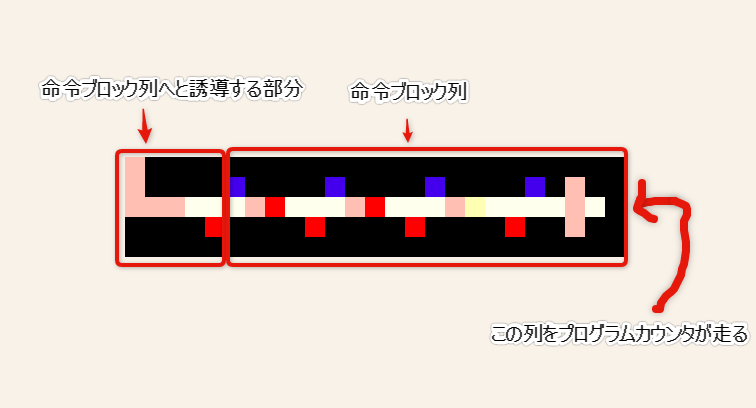
\includegraphics[width=\textwidth]{images/783f2ae98363220ed6859c9bd97cb4ff.png}} \\
赤と青のポッチは接続方向を表すマーカなので、
本質的には不要なので無視してください。

一直線のブロックの列だと、分岐もループもできず、
つまり構造化定理の順次しか実現できないので、
殆どのプログラムを書くことは出来ません。 この時点でHello
worldは書けますね。

で、次は分岐を作るわけですが、 Pointerという良い命令がPietにはあって、
それを使うとDP、つまり進む向きを変えられます。 Notという命令もあって、
それを使うとスタックの先頭が0の時だけ先頭を1に変え、
それ以外の時は先頭を0に変えられます。
Pointer命令はスタックのトップの値を見て、
その数だけDPを時計回りに回します。
これを使えば、スタックの先頭が0の時に分岐するようなものが作れます。

\href{https://gyazo.com/3c7bc0cb0dd41680c6b652ef4486b390}{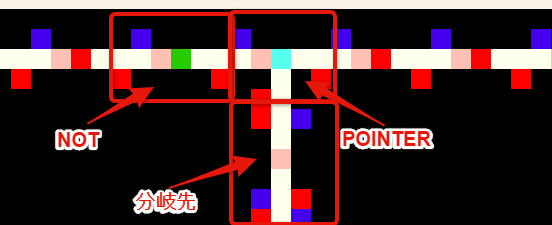
\includegraphics[width=\textwidth]{images/3c7bc0cb0dd41680c6b652ef4486b390.png}} \\
スタックの先頭が0以外の時はそのまま直進し、
0の時は下に分岐します。

これで分岐することには成功したので、
適当なところに合流したいと思います。

\href{https://gyazo.com/4f893a8b1a52e2de3f9bd70338ebb9b8}{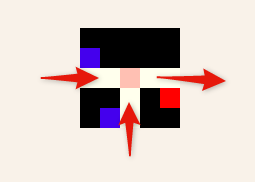
\includegraphics{images/4f893a8b1a52e2de3f9bd70338ebb9b8.png}} \\
このような構造でプログラムカウンタが下から来た場合と左から来た場合に合流してともに右に流すことができるので、
ここに飛んで来るジャンプのようなものが書けて、
あとはすぐにわかる構造で、以下の様な後ろ向きへの条件付きジャンプができます。

\href{https://gyazo.com/846e9f87a072a65e02e6943e20adc534}{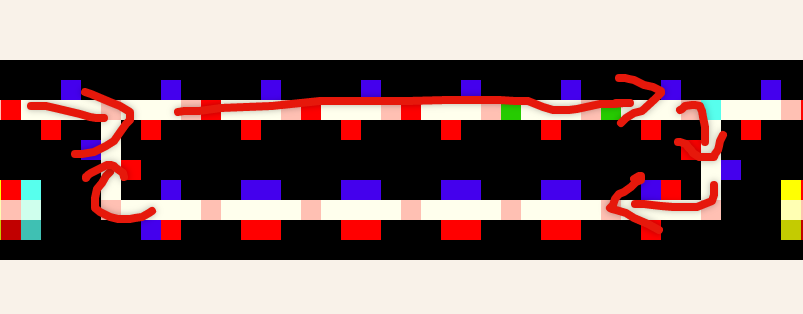
\includegraphics[width=\textwidth]{images/846e9f87a072a65e02e6943e20adc534.png}}


\end{document}
